\documentclass[tikz,margin=2mm]{standalone}

\newcommand*{\m}{\mathsf{m}}

\usetikzlibrary{trees,arrows}


\begin{document}

  		 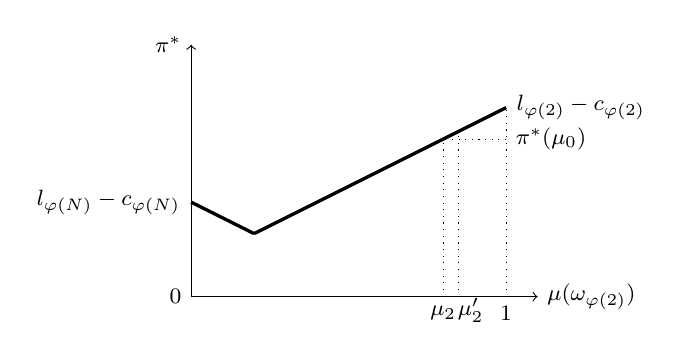
\begin{tikzpicture}[domain=0.001:1, scale=4, xscale=1,font=\footnotesize] 
  		%% vertices
    	\draw[->] (0,0) node[left]{$0$} -- (1.1,0) node[right] {$\mu (\omega_{\varphi(2)})$}; 
    	\draw[->] (0,0) -- (0,0.8) node[left] {$\pi^*$};

    	%% pi^m
    	\draw[very thick] (1,0.6) node[right]{$\color{black}l_{\varphi(2)} - c_{\varphi(2)}$} -- (0.2, 0.2);	
    	\draw[very thick] (0,0.3) node[left]{$\color{black}l_{\varphi(N)} - c_{\varphi(N)}$} -- (0.2,0.2);	

    	
%    	%% quasiconcave
%    	%% m
    	% \draw[thick, dashed] (0, 0.3) -- (0.4,0.3);	
%    	%% s
%    	\draw[thick, blue] (0.5,0.3)  -- (1,0.7) ;	
%    	\draw[dotted] (0.5,0) node [below] {$\frac{c(a_2) - c(a_1)}{l(\omega_2) - l(\omega_1)}$} -- (0.5,0.3);

        %%% pi^*(\mu_0)
    	\draw[dotted] (1,0.5) node[right]{$\pi^*(\mu_0)$} -- (0.8, 0.5);
    	\draw[dotted] (0.8,0) node[below]{$\mu_2$} -- (0.8, 0.5);
    	
    	\draw[dotted] (0.85,0) node[below,xshift=0.15cm,yshift=0.1cm]{$\mu_2'$} -- (0.85, 0.53);

    	

    	%% labels
   	\draw[dotted] (1,0) node [below]{$1$}-- (1,0.6);
%    	\draw[->] (0.12,0.15) node [below, xshift=0.5cm] {$\bar p_1(q) - c(a_1)$}-- (0.15,0.2); 
%    	\draw[->] (0.8,0.36) node [below] {$\bar p_2(q) - c(a_2)$}-- (0.78,0.48); 
    	
       	\end{tikzpicture}
       	
\end{document}